\chapter{Optimising Jastrow Factors for the Transcorrelated Method}
  \label{chap:opt}

This chapter is based in large part on the following paper:\\
\fullcite{hauptOptimizing2023}

Images have been reused from this paper (with permission).

\section{Introduction}

In this chapter, we investigate the use of flexible Jastrow factors and a novel optimisation strategy for use in \gls{TC} as introduced in section \ref{sec:tc}. As a brief recapitulation, the TC method amounts to a similarity transformation of the Hamiltonian $\hat H$, $\htc = \e^{-J}\hat H\e^J$. However, as this is a non-unitary trasformation, methods used to solve $\htc$ are in general not variational, and hence we are not guaranteed to converge to the \gls{CBS} limit from above. It is therefore important to choose $J$ wisely, as otherwise the method may be highly non-variational, and we may suffer from poor error cancellation.

As an illustration of the method, we compute the all-electron atomisation energies for the challenging first-row molecules C$_2$, CN, N$_2$ and O$_2$ and find that \gls{TC}-\gls{FCIQMC} (that is, \gls{FCIQMC} performed on a transcorrelated Hamiltonian) yields chemically accurate results using only a \vtz basis, which requires a much larger \vxz{5} basis for non-TC.

\section{Computational Details}
We compute the ground-state energies of the all-electron C, N, and O atoms, as well as that for the C$_2$, CN, N$_2$ and O$_2$ molecules at their equilibrium geometries,\todo{citations} listed in table
\ref{table:bond_lengths}.
TC- and non-TC-FCIQMC calculations used \gls{HF} orbitals (restricted open-shell in the case of open-shell systems) expanded in the standard \vxz{X} family of basis sets.\todo{cite dunning 1992}


\begin{table}[htbp]
    \centering
      \caption{
      Electronic ground states and equilibrium bond lengths used for the
      molecules considered in this work, following Ref.\
      \todo{citation}.
    }
    \label{table:bond_lengths}
    \begin{tabular}{ccc}
      System & State & $r_\mathrm{eq}$ (\AA) \\
    \hline \hline
      C$_2$ & ${}^1\Sigma_g^+$ & $1.2425$ \\
      CN    & ${}^2\Sigma^+$   & $1.1718$ \\
      N$_2$ & ${}^1\Sigma_g^+$ & $1.0977$ \\
      O$_2$ & ${}^3\Sigma_g^-$ & $1.2075$ \\
    \hline
    \end{tabular}
\end{table}

The quality of the energy differences is assessed using the atomisation energies of these molecules. In order to determine if our methodology yields chemically-accurate, i.e. within an error of $1$ kcal/mol $\approx 1.6$ mHa, we also keep each individual error to be well within this threshold. We expect a total bias in our resulting relative energies of not more than $0.5$ mHa.

For all our calculations, we generate our orbitals and integration grids using \pyscf,\supercite{sunPySCF2018} optimise the Jastrow factors using the \casino continuum \gls{QMC} package,\supercite{needsVariational2020}, compute TC matrix elements using the \tchint library, for which more details are presented in appendix \ref{chap:pytchint}, and perform (TC-)FCIQMC calculations using the \neci package.\supercite{gutherNECI2020} FCIQMC energies reported are the standard HF-projected energies.

(TC-)FCIQMC values presented here were produced using a walker-number extrapolation scheme presented in another dissertation.\todo{cite Mohammadreza}

\section{Jastrow Factor}

In continuum quantum Monte Carlo methods, the Jastrow factor for a molecule is typically expressed as the sum of electron-electron, electron-nucleus, and electron-electron-nucleus terms,\footnote{Of course, these are not all the possible terms. We may, for example, also choose to include electron-nucleus-nucleus terms.}
\begin{equation}
    \label{eq:jastrow}
    J = \sum_{i<j}^Nv(r_{ij}) + \sum_i^N\sum_I^{N_A}\chi(r_{iI}) + \sum_{i<j}^N\sum_I^{N_A}f(r_{ij}, r_{iI}, r_{jI}),
\end{equation}
where $N_A$ is the number of nuclei, $N$ the number of electrons, and each of $u$, $\chi$, and $f$ are expressed as natural power expansions.\supercite{drummondJastrow} That is,
\begin{equation}
    \label{eq:dtn-jastrow-ee}
    v(r_{ij})    = t(r_{ij},L_v)
                    \sum_{k} a_k r_{ij}^k ,
\end{equation}
\begin{equation}
    \label{eq:dtn-jastrow-en}
    \chi(r_{iI}) = t(r_{iI},L_\chi)
    \sum_{k} b_k r_{iI}^k ,
\end{equation}
\begin{equation}
    \label{eq:dtn-jastrow-een}
    f(r_{ij}, r_{i}, r_{j}) = t(r_{iI},L_f) t(r_{jI},L_f)
    \sum_{k,l,m} c_{klm}
    r_{ij}^k r_{iI}^l r_{jI}^m ,
\end{equation}
where $\{a_k\}$, $\{b_k\}$, and $\{c_{klm}\}$ are linear parameters,
$L_v$, $L_\chi$, and $L_f$ are cut-off lengths, $t(r,L) = (1-r/L)^3
\Theta(r-L)$ is a cut-off function, and $\Theta(r-L)$ is the Heaviside
step function.

As described in chapter \ref{chap:explicit}, accurately describing the (electron-electron and electron-nucleus) Kato cusp conditions\supercite{katoEigenfunctionsManyparticleSystems1957a} substationally improves the accuracy of our method. Also, as described in chapter \ref{chap:qmc}, \gls{VMC} and \gls{DMC} methods sample electronic configurations $\{\bm R\}$ from a probability distribution based on an analytical trial wave function $\tilde\Psi_{\mathrm T}(\bm R)$ to produce a variational estimate of the total energy as an average of the local energy, $E_{\mathrm L}({\bm R}) = \tilde\Psi_{\mathrm T}^{-1}({\bm R}) \hat H({\bm R}) \tilde\Psi_{\mathrm T}({\bm R})$ over the sampled configurations. In the case of \gls{VMC}, accurate description of the electron-electron and electron-nucleus Kato cusp conditions suppresses extreme outliers in the local energy sampling, allowing meaningful wave function parameters.

The most obvious way to enforce the electron-electron and electron-nucleus cusp conditions is by enforcing them in the form of the Jastrow factor through the relevant terms, namely $v$ (equation \ref{eq:dtn-jastrow-ee}) for the electron-electron cusp, and $\chi$ (equation \ref{eq:dtn-jastrow-en}) for the electron-nucleus cusp. However, in the context of continuum \gls{QMC}, it has been found to be better\supercite{drummondJastrow,needsVariational2020,maScheme2005} to enforce the electron-nucleus cusp by modifying the $l=0$ ($s$-type) component of the cuspless molecular orbitals, $\phi(r)$, such that they exhibit a cusp.

Since we are interested in performing a post-Hartree-Fock calculation on $\htc$, such as \gls{FCIQMC}, it is preferable to use unmodified molecular orbitals from standard basis sets during the optimisation process. If we optimise the Jastrow factor in \gls{VMC} in the presence of cusp-corrected orbitals and then use them in TC-FCIQMC without the cusp-corrected orbitals, the Jastrow factor would be sub-optimal for the Hamiltonian, by construction.

Instead, we recast the cusp-correction scheme of \onlinecite{maScheme2005} as an electron-nucleus Jastrow factor term, called $\Lambda$, to be added (rather than replacing) the $\chi$ term of equation \ref{eq:dtn-jastrow-en}. We construct this term as

\begin{equation}
    \label{eq:cusp-corr-1}
    \Lambda(r)  = \left[ \ln \tilde \phi(r) - \ln \phi(r) \right]\Theta(r-r_{c}),
\end{equation}
where, adopting the notation of \onlinecite{maScheme2005}, $r_c$ is a cutoff radius, $\phi(r)$ is the $s$-type component of the target orbital, and $\tilde \phi(r)$ is its cusp-corrected counterpart,
\begin{equation}
    \label{eq:cusp-corr-2}
  \tilde \phi(r) = \e^{\sum_{l=0}^4 \alpha_l r^l} + C \quad,\quad r<r_{c}.
\end{equation}

Here, $\{\alpha_l\}$ are parameters determining the shape of the
corrected orbital and the shift $C$ is only set to a non-zero value in
the presence of nodes of $\phi(r)$ near the nucleus. More precisely, the shift $C$ is chosen such that $\tilde\phi(r_c)-C$ is of one sign within the radius $r_c$. This is necessary since we wish to impose an exponential correction, which is necessarily of one sign.

Following \onlinecite{maScheme2005}, we impose the cusp condition at $r=r_c$, as well as twice continuous differentiability at $r=r_c$. This leaves only $\alpha_0$ and $r_c$ as free parameters from equations \ref{eq:cusp-corr-1} and \ref{eq:cusp-corr-2}. $r_c$ is chosen to be small but within the same sign, as described above, while $\alpha_0$ is determined by enforcing smoothness for the so-call ``effective one-electron local energy'',
\begin{equation}
    E_L^s(r) \mathdef \tilde\phi(r)^{-1}\left[-\frac 12\nabla^2-\frac{Z_{\mathrm{eff}}}r\right]\tilde\phi(r).
\end{equation}
Here, the effective nuclear charge $Z_\mathrm{eff}$,
\begin{equation}
    Z_\mathrm{eff} = Z\left(1 + \frac{\eta(0)}{\tilde\phi(0)}\right)
\end{equation}
ensures that $E_L^s$ is finite at the origin, and is derived from the cusp condition. $\eta$ is the rest of the orbital, leftover from removing the $s$-type component.

Figure \ref{fig:cusp-term} illustrates the effect of using a $\Lambda$
term in practice.

\begin{figure}[htbp]
    \centering
    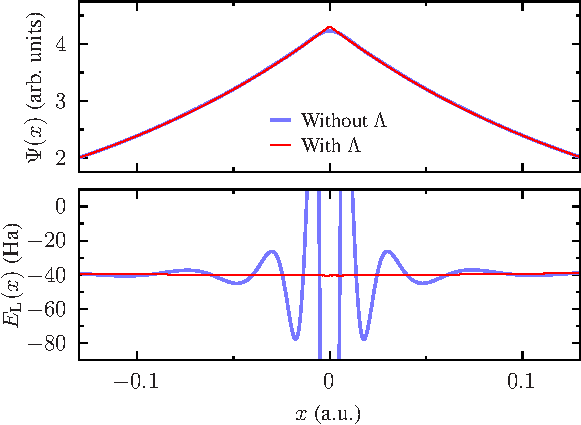
\includegraphics[width=0.8\columnwidth]{figures/optimisation/Fig/cusp-term-eps-converted-to}
    \caption{\gls{HF} wave function value and local energy as a function of the $x$ coordinate of an electron in a carbon atom as it crosses the nucleus at $x=0$, both with and without the $\Lambda$ cusp-correcting Jastrow factor term. This is in the \vdz basis.}
    \label{fig:cusp-term}
\end{figure}

For the calculations in this chapter, we use a total of $44$ optimisable Jastrow factor parameters for the atoms and homonuclear dimers, and $88$ parameters for CN. We keep the $L_v$, $L_\chi$ and $L_f$ cutoff lengths fixed at $4.5$, $4$, and $4$, for simplicity.

\section{Optimisation Strategy}

We optimise $J$ using \gls{VMC}. VMC provides a variational framework in which parameters $\bm \alpha$ present in a trial wave function $\Psi_\mathrm{T}$ can be optimised. In this chapter, $\ket{\Psi_\mathrm{T}} = \e^{J(\bm\alpha)}\ket{D_\mathrm{HF}}$.

Wave function optimisation is usually carried out using a correlated-sampling approach in which a set of $n_mathrm{opt}$ electronic real-space configurations ${\{\bm R}_{i}\}_{i=1}^{n_\mathrm{opt}}$ distributed according to the initial wave function squared, $|\Psi_\mathrm{T}({\bm R}; {\bm \alpha}_0)|^2$ is generated, and then a target function is minimised by varying $\bm\alpha$ at fixed ${\{\bm R}_{i}\}$.

The variational energy estimate for this trial wave function may be written
\begin{equation}
    E_\mathrm{VMC} = \frac{\bra{\Psi_\mathrm{T}} \hat H \ket{\Psi_\mathrm{T}} }{ \braket{\Psi_\mathrm{T}}{\Psi_\mathrm{T}} },
\end{equation}
which may be used as a target function, as presented in section \ref{sec:vmc}.

Another popular target function is the ``variance of the VMC energy,''\todo{citations}
\begin{equation}
\sigma_\mathrm{VMC}^2 = \frac{\bra{\Psi_\mathrm{T}}(\hat H - E_\mathrm{VMC})^2\ket{\Psi_\mathrm{T}}}{\braket{\Psi_\mathrm{T}}},
\end{equation}
which reaches its minimum of zero when the trial wave function is an eigenstate of the Hamiltonian. In practice, minimising $\sigma_\mathrm{VMC}^2$ yields variational energies, but is affected by large fluctuations, as shown in this chapter.

In continuum QMC methods, modifications have been devised to
circumvent this problem, such as weight limiting, unreweighted
variance minimization, or the minimization of other measures of spread
such as the median absolute deviation from the median energy.\supercite{needsVariational2020}

The computational cost of optimizing Jastrow factors within VMC scales
as a small power of system size, typically estimated to be ${\mathcal
O}(N^3)$.

\subsection{Variance of the Reference Energy Minimisation}

In the context of TC, the reference energy
\begin{equation}
    E_\mathrm{ref} = \bra{D_\mathrm{HF}}\e^{-J}\hat H\e^J\ket{D_\mathrm{HF}}
\end{equation}
is of particular significance since it represents the starting point of a TC-FCIQMC calculation (i.e. the walker distributions at imaginary time $\tau=0$ has this energy). It is also the zeroth-order contribution to the TC-\gls{CC} energy.

We refer to its associated variance,
\begin{equation}
  \label{eq:var_eref_1}
  \sigma_\mathrm{ref}^2 =
    \bra{D_\mathrm{HF}}\e^{-J} (\hat H^\dag-E_\mathrm{ref})(\hat H-E_\mathrm{ref}) \e^J\ket{D_\mathrm{HF}}
\end{equation}
as the ``variance of the reference energy,'' which is easily evaluated for a finite VMC sample of size $n_\mathrm{opt}$ as the sample variance of the Slater-Jastrow energy over the HF distribution,
\begin{equation}
    S_\mathrm{ref}^2 =
      \frac 1 {n_\mathrm{opt}-1}
      \sum_{n=1}^{n_\mathrm{opt}}
        \left| \frac {\hat H({\bm R}_n) \Psi_\mathrm{SJ}({\bm R}_n)}
                     {\Psi_\mathrm{SJ}({\bm R}_n)} - {\bar E}_\mathrm{ref}
        \right|^2,
\end{equation}
% TODO : you will want to practice proving this, just in case for your defence
which tends to $\sigma_\mathrm{ref}^2$ as $n_\mathrm{opt}\to\infty$, where $\Psi_\mathrm{SJ}\mathdef \e^JD_\mathrm{HF}$ is the Slater-Jastrow wave function, $\{{\bm R}_n\}_{n=1}^{n_\mathrm{opt}}$ are electronic
configurations distributed according to $D_\mathrm{HF}^2$, and the VMC
estimate of the reference energy is
\begin{equation}
    {\bar E}_\mathrm{ref} =
      \frac 1 {n_\mathrm{opt}}
      \sum_{n=1}^{n_\mathrm{opt}}
        \frac {\hat H({\bm R}_n) \Psi_\mathrm{SJ}({\bm R}_n)}
              {\Psi_\mathrm{SJ}({\bm R}_n)}.
\end{equation}

% TODO: you will want to familiarise yourself with these papers
The variance of the reference energy has been used as a target function for optimising Jastrow factors for the TC method before, albeit in different theoretical frameworks.\todo{citations}

To understand the physical significance of the variance of the reference energy, note that equation \ref{eq:var_eref_1} may be rewritten as
\begin{equation}
    \label{eq:varref-connectivity}
    \sigma_\mathrm{ref}^2 = \sum_{I\neq \mathrm{HF}}\bra{D_I}\htc\ket{D_\mathrm{HF}},
\end{equation}
where $I$ runs over a complete basis set.\footnote{Here we have a complete basis set because we are optimising with continuum Monte Carlo. If we were to optimise this by directly calculating the matrix elements in equation \ref{eq:varref-connectivity}, then the sum must be truncated. This is the subject of ongoing work.}

As evident by equation \ref{eq:varref-connectivity}, minimising $\sigma_\mathrm{ref}^2$ essentially amounts to minimising the coupling of the reference determinant with the remainder of the space, which in the context of FCIQMC translates to a reduced spawning rate from the reference determinant to its connected excited-state determinants, thereby increasing the amplitude of the reference determinant in the resulting CI vector.

Note also that if the Slater-Jastrow wave function were an exact eigenstate of $\hat H$, then a TC-FCIQMC simulation starting from the HF determinant would immediately converge to a strictly single-determinant solution. Although this ideal scenario cannot be achieved in practice, it nevertheless illustrates the potential benefits of obtaining a relatively single-reference CI solution by minimising this target function. We expect that this increased single-reference character will also benefit other approaches, particularly those based on single references, such as TC-CC.

We therefore investigate the performance of minimising the variance of the reference as an alternative to minimising the variance of the VMC energy. In figure \ref{fig:varmin-E-Eref}, we compare the VMC energy and variance obtained by variance minimisation methods along with energy-minimised \todo{citations} results for reference, for the systems considerd in this chapter, using $n_\mathrm{opt}=10^5$ VMC configurations.

\begin{figure}[htbp]
    \centering
    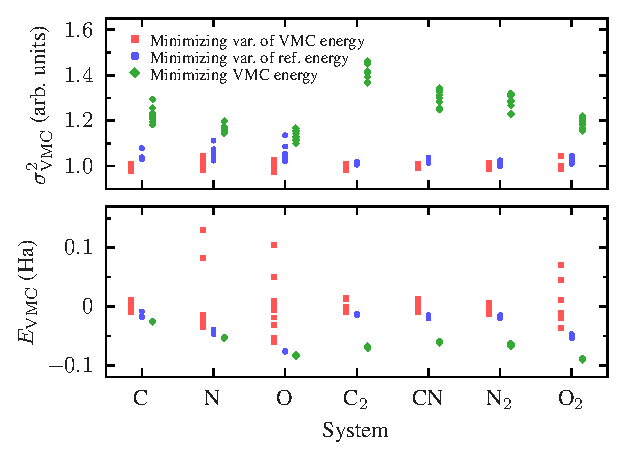
\includegraphics[width=0.8\textwidth]{figures/optimisation/Fig/varmin-E-Eref}
    \caption{Variance of the VMC energy (top) and VMC energy (bottom) of the systems considered in this chapter using the \vtz basis and Jastrow factors obtained by minimising the variance of the VMC energy (red squares), the variance of the reference energy (blue circles), or the VMC energy (green diamonds) in each of ten independent optimisation runs with $n_\mathrm{opt}=10^5$ VMC configurations. To ease comparisons, variances have been rescaled and energies shifted by their average values from minimising the variance of the VMC energy (i.e. the red squares average to a variance of $1$ and an energy of $0$ in the plot). The subpar ability of VMC energy variance minimisation to yield consistent VMC energies is evident in the bottom panel, suggesting to use the variance of the reference.}
    \label{fig:varmin-E-Eref}
\end{figure}
%
Minimizing the variance of the VMC energy produces lower average
values of $\sigma_\mathrm{VMC}^2$, as one would expect, but also erratic
VMC energies with very large standard deviations (up to $\sim50$ mHa
in our tests).
%
Minimizing the variance of the reference energy, on the other hand,
produces values of $\sigma_\mathrm{VMC}^2$ which are only slightly higher
on average than those obtained from minimizing the variance of the VMC
energy ($1$--$5\%$ in our tests), while producing more stable VMC
energies with much smaller standard deviations (up to $\sim3$ mHa in
our tests).
%
We therefore do not use ``regular'' variance minimization since it
introduces large stochastic noise, making it unsuitable for optimizing
Jastrow factors, and from this point on we use the term ``variance
minimization'' to refer to the minimization of the variance of the
reference energy.

\subsection{Choosing an Appropriate Sample Size}

While expectation values relevant for most continuum QMC calculations converge using relatively few VMC configurations, it has also been known\todo{citation Spink} that in order to converge other quantities, far more configurations are needed. That is, $n_\mathrm{opt}$ is larger. In the spirit of \gls{MC}, we may estimate the convergence of the expectation value for some quantity by performing multiple optimisation runs with different random number seeds but otherwise the same inputs. This would give us a standard deviation.

The value we want to converge in this case is not the VMC energy, nor the reference energy, but instead the TC-FCI energy. In practice, we use the uncertainty of the VMC estimate of the reference energy $\bar E_\mathrm{ref}$ as a proxy for the standard deviation of the TC-FCIQMC energy. This is justified because:
\begin{itemize}
    \item The standard deviation of the TC-FCIQMC energy is not larger than the standard deviation of the reference energy, as illustrated in figure \ref{fig:spread_c2_cc-pvdz}. It is usually significantly smaller thanks to the ability of TC-FCIQMC to conpensate for the presence of a bias in $E_\mathrm{ref}$ via the correlation energy.
    \item The standard deviation of the reference energy is not larger than the statistical uncertainty of the VMC estimate of the reference energy obtained with $n_\mathrm{opt}$ configurations. It is usually significantly smaller due to the use of variance reduction techniques in QMC.
\end{itemize}

\begin{figure}[htbp]
    \centering
    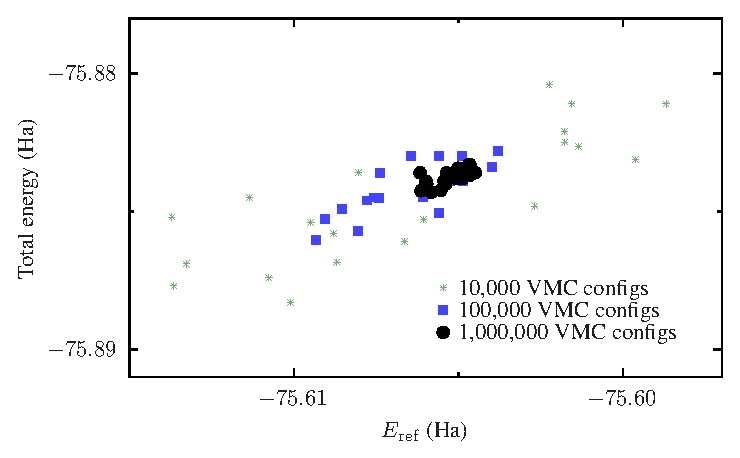
\includegraphics[width=0.8\textwidth]{figures/optimisation/Fig/spread_c2_cc-pvdz}
    \caption{TC-FCIQMC energy of the C$_2$ molecule using $10^6$ walkers with the \vdz basis as a function of the reference energy for multiple independent Jastrow factor parameter sets obtained by variance minimisation using three different VMC sample sizes. The horizonal spread is about $1.8$ times larger than the vertical spread, in line with the expectation that the standard deviation of the TC-FCIQMC energy is smaller than that of the reference energy.}
    \label{fig:spread_c2_cc-pvdz}
\end{figure}

For the atoms and molecules considered in this chapter, we use $n_\mathrm{opt}=2\times 10^7$ to yield TC-FCIQMC energies with standard deviations of less than $0.1$ mHa.

\subsection{Energy Minimisation}

\todo{...}


\section{Grid Sizes}
\todo{discuss the grid size (section III.C)}
\todo{...}


\section{Compactification of the CI Vector}
\todo{talk about compactness}

\section{Atomisation Energies}

\section{Neglecting Three-Body Excitations}

\todo{...}
\todo{mention Pauli exclusion principle as an argument for why this is a valid approximation (maybe use a figure?)}

\section{Conclusion and Outlook}
\todo{mention this is the way we now optimise Jastrow factors, but there is an important extension to the no-3-body approximation, xTC. Briefly describe.}
\todo{...}

\subsection{The xTC Approximation}

\todo{...}

\label{sec:xtc}
